\section{Messungen mit dem Szintillationszähler}

\subsection{Messung des Gammaspektrums}

\subsubsection{Aufbau}

\begin{minipage}{0.5\textwidth}
\begin{figure}[H]
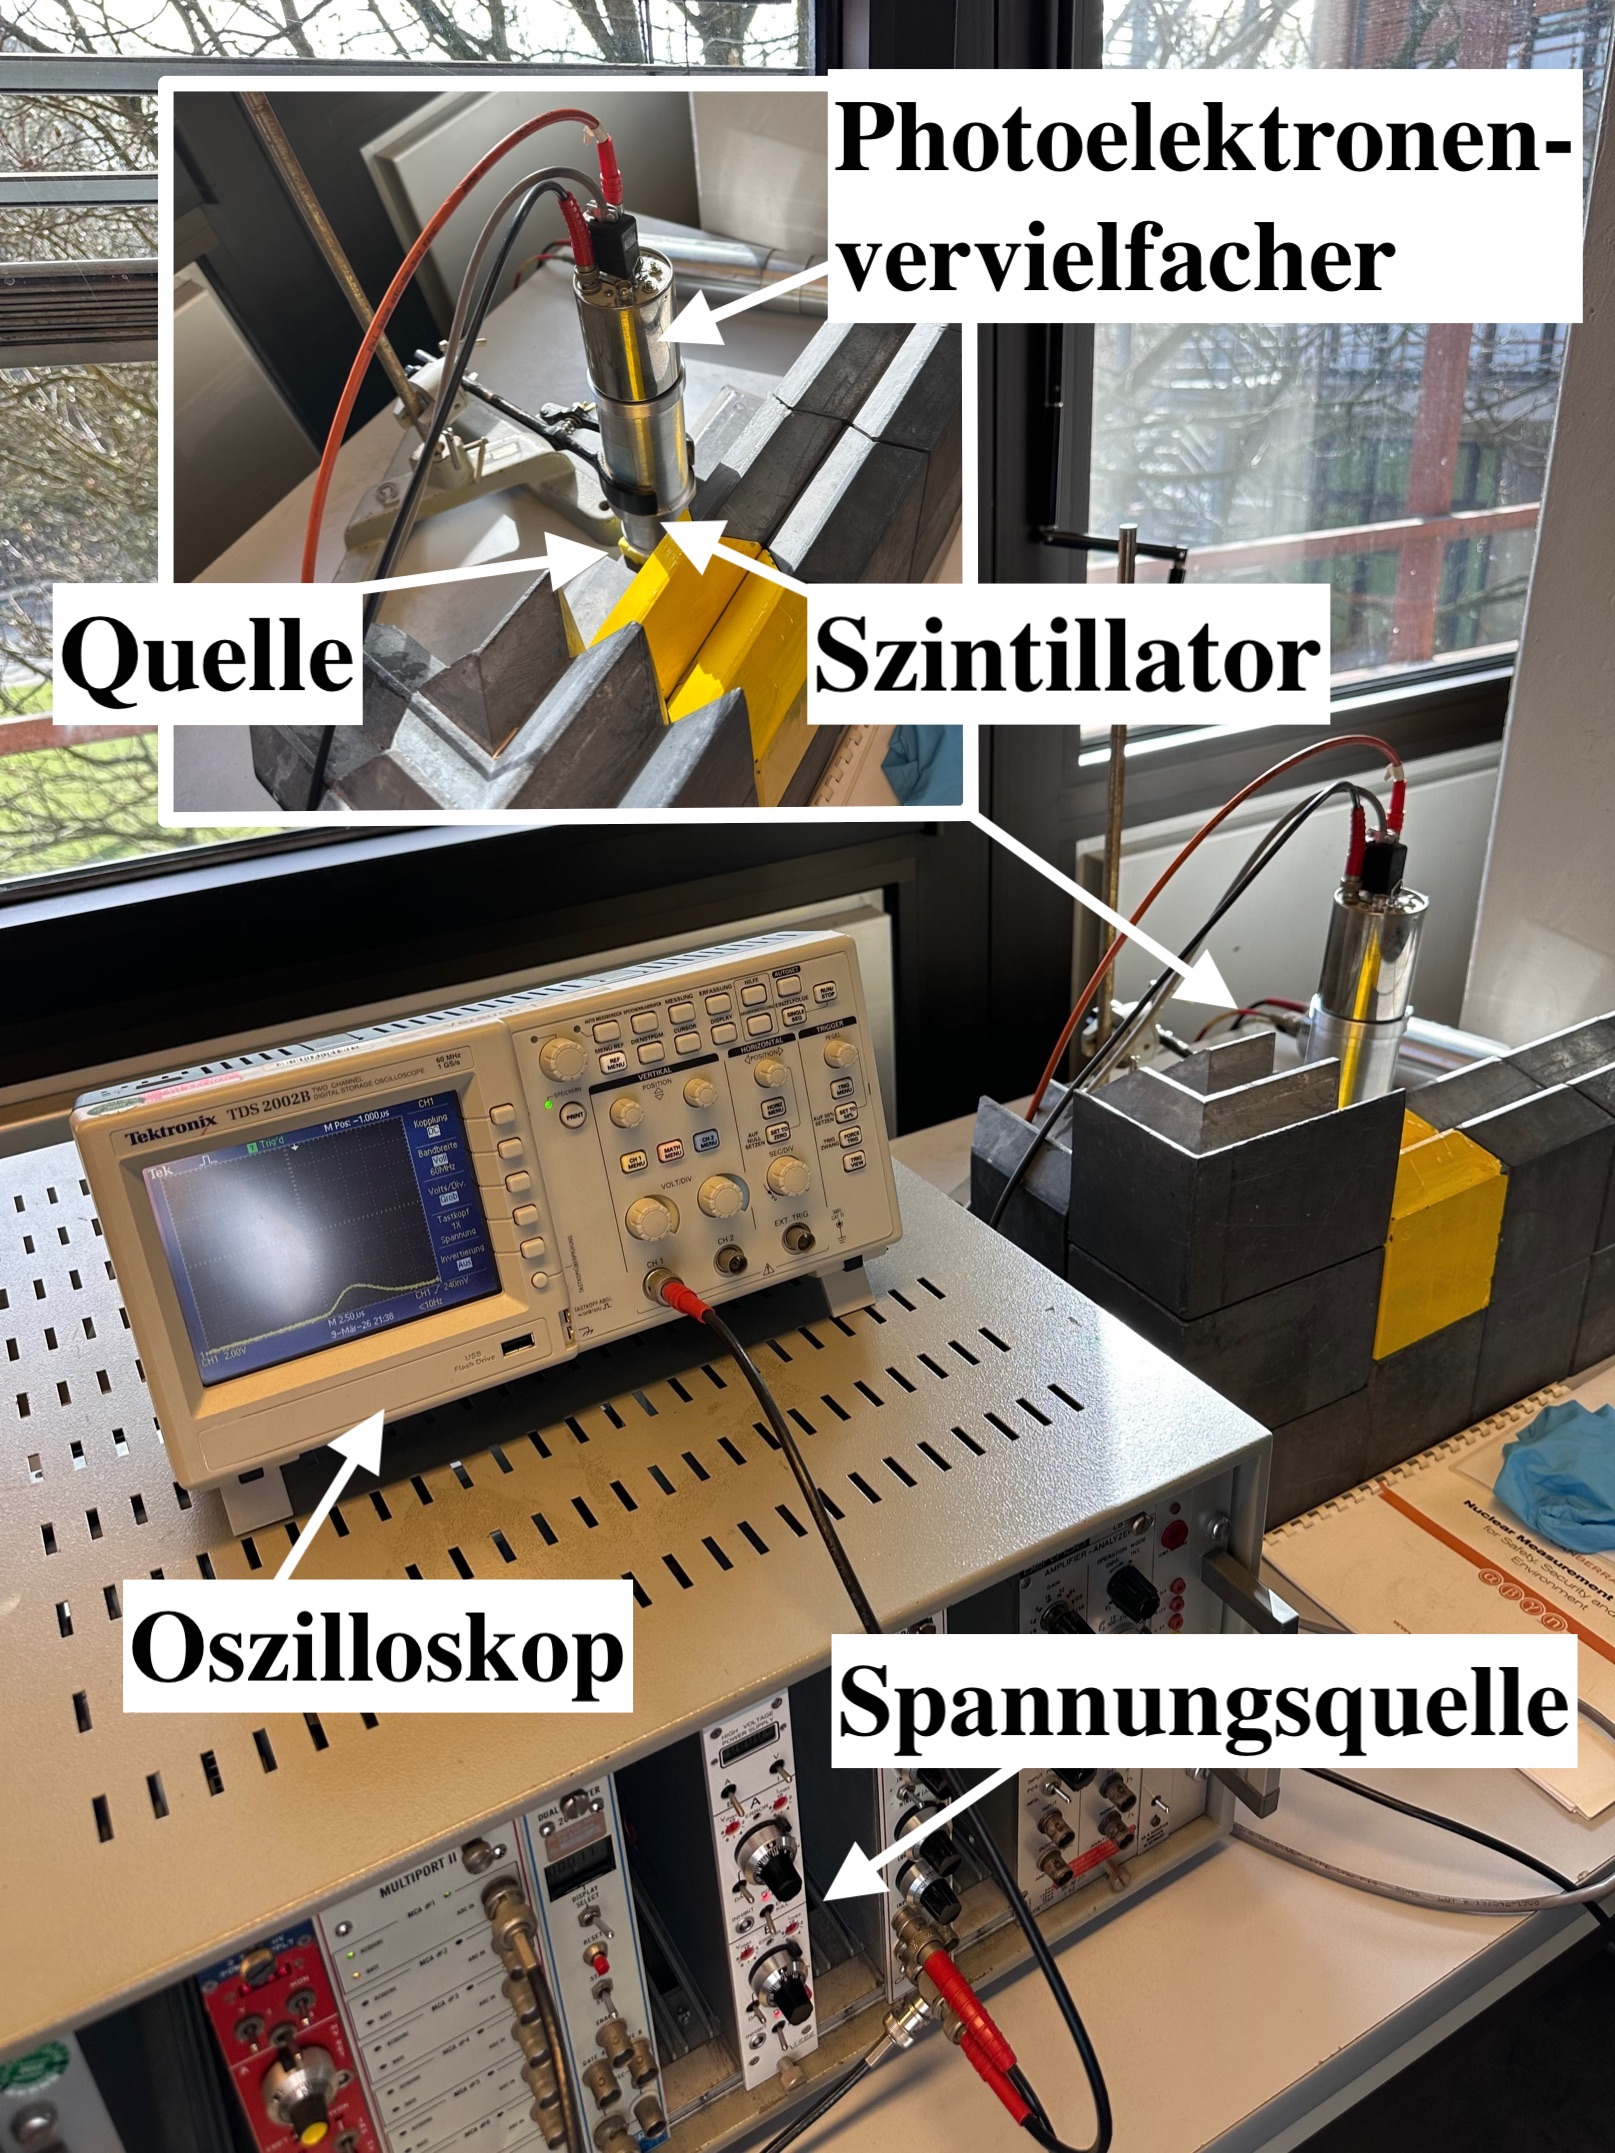
\includegraphics[width = 1\textwidth]{Bilder/Aufbau_Gamma_2_Szintillatoren.jpeg}
\caption{\label{fig:Aubau_Gamma_2_Szinti} Aufbau}
    \end{figure}
\end{minipage} \hfill
\begin{minipage}{0.45\textwidth}

Der Aufbau besteht aus zwei Szintillatoren (NaI(Tl) und Plastik), mit denen nacheinander die gleiche Quelle $^{137}$Cs vermessen wurde. Der Szintillator ist an einem Photoelektronenvervielfacher angebracht, der wiederum mit der Spannungsquelle verbunden ist und mit einem NIM-Modul zur Auslese am Oszilloskop. Außerdem gab es eine Verbindung zum PC zur Auswertung der Pulshöhenspektren.

\end{minipage}

\subsubsection{Messung und Ergebnisse}

Folgende Messeinstellungen haben wir für die Spektrenvermessung festgelegt: 
\begin{table}[h]
    \centering
    \begin{tabular}{|c|c|c|}
        \hline
        untere Schwelle & Spannung & Messzeit \\
        \hline 
        \SI{1.5}{\%} & \SI{800}{\V} & \SI{600}{\sec} \\
        \hline 
    \end{tabular}
    \label{tab: Messeinstellungen Gamma 2 Szinti}
\end{table}

\subsection{Absorption von Gammastrahlung in Blei}

\subsubsection{Aufbau}

\begin{minipage}{0.5\textwidth}
\begin{figure}[H]
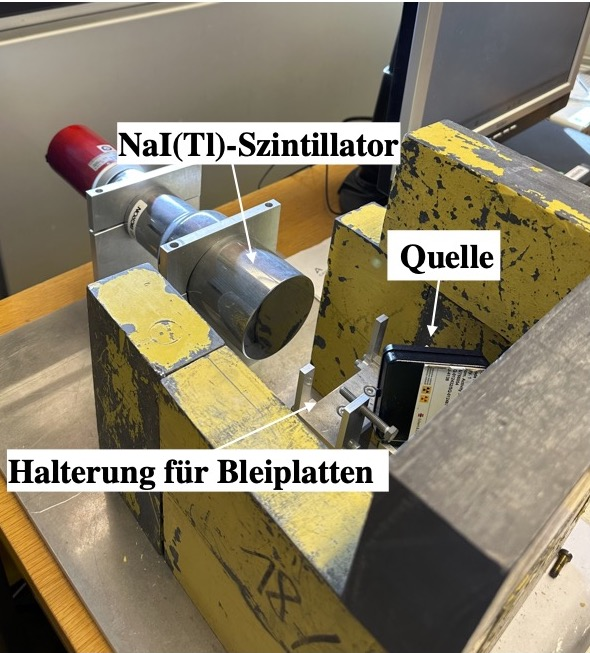
\includegraphics[width = 1\textwidth]{Bilder/Aufbau_Gamma_Blei.jpeg}
\caption{\label{fig:Aubau_Gamma_Blei} Aufbau}
    \end{figure}
\end{minipage} \hfill
\begin{minipage}{0.45\textwidth}

Der Aufbau besteht aus einem NaI(Tl)-Szintillator, einer $^{137}$Cs-Quelle und Bleiplatten mit verschiedenen Dicken, die zwischen der Quelle und dem Szintillator platziert werden. Zusätzlich ist der gesamte Aufbau abgeschirmt. Der Szintillationszähler ist direkt mit dem Auswertungsprogramm Genie2000 verbunden.
\end{minipage}



\subsubsection{Messdurchführung und -ergebnisse}

Zuerst haben wir die für die Messung verwendeten Bleiplatten mehrfach vermessen, um Unsicherheiten in der Dicke der Abschirmung abschätzen zu können (vgl. Tabelle \ref{tab: Messung Bleiplatten}). 

\begin{table}[h]
    \centering 
    \resizebox{\textwidth}{!}{
    \begin{tabular}{|l|c|c|c|c|c|c|}
        \hline 
        angegebene Dicke & \SI{1}{\mm} & \SI{2}{\mm} & \SI{3}{\mm} & \SI{5}{\mm} & \SI{10}{\mm} & \SI{20}{\mm} \\
        \hline 
         & \SI{0.95}{\mm} & \SI{1.95}{\mm} & \SI{2.95}{\mm} & \SI{4.90}{\mm} & \SI{9.95}{\mm} & \SI{19.95}{\mm} \\ 
        vermessene Dicke & \SI{1.00}{\mm} & \SI{2.00}{\mm} & \SI{3.00}{\mm} & \SI{4.90}{\mm} & \SI{9.95}{\mm} & \SI{20.00}{\mm} \\ 
         & \SI{0.90}{\mm} & \SI{1.95}{\mm} & \SI{2.90}{\mm} & \SI{4.95}{\mm} & \SI{9.95}{\mm} & \SI{20.00}{\mm} \\
        \hline   
        gemittelte Dicke & 0.95$\pm$\SI{0.05}{\mm} & 1.97$\pm$\SI{0.03}{\mm} & $2.95\pm$\SI{0.05}{\mm} & $4.92\pm$\SI{0.03}{\mm} & $9.95\pm$\SI{0.01}{\mm} & $19.98\pm$\SI{0.03}{\mm} \\ 
        \hline 
    \end{tabular}
    }
    \caption{Die gemittelten Dicken wurden über das arithmetische Mittel der gemessenen Dicken gebildet und die Unsicherheit über die Stichprobenvarianz quadratisch addiert mit der Ablesegenauigkeit von \SI{0.05}{\mm} geteilt durch $\sqrt{12}$  bestimmt.}
    \label{tab: Messung Bleiplatten}
\end{table}

Anschließend haben wir mit dem Szintillator mehrmals das $^{137}$Cs-Spektrum vermessen mit unterschiedlich dicken Bleiplatten zwischen Quelle und Szintillator. Unsere Messeinstellungen sind in Tabelle \ref{tab: Messeinstellungen Gamma Blei} aufgeführt. 

\begin{table}[h]
    \centering
    \begin{tabular}{|c|c|c|c|}
        \hline
        untere Schwelle & Spannung & Messzeit & Gain \\
        \hline 
        Auto & \SI{700}{\V} & \SI{400}{\sec} & 2.0 \\
        \hline 
    \end{tabular}
    \label{tab: Messeinstellungen Gamma Blei}
\end{table}

In Abbildung \ref{fig:Gesamtspektrum Gamma Blei} ist das aufgenommene Gesamtspektrum ohne Bleiabschirmung dargestellt. Im Spektrum ist der Effekt des nebenstehenden Mößbauer-Versuchs sichtbar, aber auch das Energiespektrum des $\gamma$-Strahlers ist gut zu erkennen. \\


\begin{figure}[h]
    \centering
    \includesvg[width=0.8\textwidth]{Bilder/Abbildungen_Gamma_Blei/Gamma_Blei_ohneAbschirmung_Spektrum.svg}
    \caption{}
    \label{fig:Gesamtspektrum Gamma Blei}
    
\end{figure}

Für die weitere Auswertung benutzen wir nur die Photopeaks der Spektren, da sich aus diesen, durch einen Gaußkurvenfit, die Intensitäten $I(x)$ bestimmen lassen, die für die Bestimmung des Absorptionskoeffizienten $\mu$ benötigt werden (vgl. Gleichung \ref{Absorptionsgesetz}). 

\begin{equation}
    I(x) = I_0e^{-\mu x} \Leftrightarrow \mu = \frac{1}{x} \cdot ln\left(\frac{I_0}{I(x)}\right)
    \label{Absorptionsgesetz}
\end{equation}

Zur Entfernung des Untergrunds wurde die Rauschmessung abgezogen und zusätzlich eine zweite Gaußkurve zum Gaußfit hinzugefügt. \\
Die Darstellung dieses Fits ist in Abbildung \ref{fig:Gamma Blei Dicke 1} für eine Absorptionsschichtdicke von \SI{20}{\mm} zu sehen. Die restlichen Fits sind im Appendix zu finden (vgl. Abbildung \ref{fig:Gamma Blei untersch. Dicken}). \\


\begin{figure}[h]
    \centering
    \includesvg[width=0.8\textwidth]{Bilder/Abbildungen_Gamma_Blei/Gamma_Blei_Plot_20.svg}
    \caption{Absorptionsschichtdicke: \SI{20}{\mm}}
    \label{fig:Gamma Blei Dicke 1}
    
\end{figure}

Der Zusammenhang zwischen $I(x)$ und dem Fit ergibt sich zu: 
\begin{center}
    $ \frac{A}{\text{Messzeit}} = I(x),  \text{ mit} \text{ Fit}=\frac{A}{\sigma_1\sqrt{2\pi}} e^{-\frac{(x - \mu_1)^2}{ 2\sigma_1^2}} + \frac{B}{\sigma_2\sqrt{2\pi}} e^{-\frac{(x - \mu_2)^2}{ 2\sigma_2^2}} $
\end{center} 


Nach Durchführung des Fits ergeben sich folgende Daten: 

\begin{table}[h] 
    \begin{tabular}{|c|c|c|c|c|}

    \hline 
    Abschirmung & $A$ & $I(x)$ in $\frac{1}{\si{\sec}}$ & $\chi^2$ & $\frac{\chi^2}{N_{dof}} $ \\
    \hline 
    \SI{0}{\mm} & 812208.23 ± 1063.24 & 2030.52 ± 2.66 & 1130.06 & $\frac{1130.06}{200-6}=5.83 $ \\ 
    \hline 
    \SI{1}{\mm} & 720885.63 ± 1046.37 & 1802.21 ± 2.62 & 892.35 & $\frac{892.35}{200-6}=4.60 $\\ 
    \hline 
    \SI{2}{\mm} & 640310.40 ± 1028.62 & 1600.77 ± 2.57 & 810.26 & $\frac{810.26}{200-6}=4.18 $ \\ 
    \hline 
    \SI{3}{\mm} & 576145.24 ± 1012.92 & 1440.36 ± 2.53 & 857.49 & $\frac{857.49}{200-6}=4.42 $ \\ 
    \hline 
    \SI{5}{\mm} & 462117.86 ± 977.67 & 1155.29 ± 2.44 & 815.45 & $\frac{815.45}{200-6}=4.20 $ \\ 
    \hline 
    \SI{10}{\mm} & 268917.90 ± 977.74 & 672.29 ± 2.44 & 478.46 & $\frac{478.46}{200-6}=2.47 $ \\ 
    \hline 
    \SI{15}{\mm} & 156476.47 ± 866.37 & 391.19 ± 2.17 & 455.20 & $\frac{455.20}{200-6}=2.35 $ \\ 
    \hline 
    \SI{20}{\mm} & 90411.38 ± 780.70 & 226.03 ± 1.95 & 316.92 & $\frac{316.92}{200-6}=1.63 $ \\ 
    \hline 

    \end{tabular}
    \label{tab: Fitergebnisse Gamma Blei}
    \caption{Aus dem Fit erhaltene Werte für die Fläche unter der Kurve, die darüber berechnete Intensität $I(x)$ und die Güte der Anpassung. Die Fehler auf $I(x)$ wurden über die Gauß'sche Fehlerfortpflanzung berechnet.}
\end{table}

Mit diesen Werten und den gemessenen Dicken $x$ der Platten (\ref{tab: Messung Bleiplatten}) können wir jetzt den Abschwächungskoeffizienten $\mu$ nach Gleichung \ref{Absorptionsgesetz} berechnen, wobei wir für $I_0$ den Intensitätswert von keiner Abschirmung nutzen.  

Damit ergeben sich für $\mu$ die folgenden Werte:


\begin{table}
\centering
    \begin{tabular}{|c|c|}
    \Xhline{1.5pt}
    \multicolumn{2}{|c|}{Berechnete $\mu$}\\ \Xhline{1.5pt}
    \SI{1}{\mm} & $2290.6\pm15.4$ \\ \hline
    \SI{2}{\mm} & $3749.2\pm3.1$ \\ \hline
    \SI{3}{\mm} & $5055.3\pm4.9$ \\ \hline
    \SI{5}{\mm} & $7808.6\pm0.5$ \\ \hline 
    \SI{10}{\mm} & $5055.3\pm4.9$ \\ \hline
    \SI{15}{\mm} & $5055.3\pm4.9$ \\ \hline
    \SI{20}{\mm} & $5055.3\pm4.9$ \\ \Xhline{1.5pt}
    \multicolumn{2}{|c|}{$\overline{\mu} = $}\\ \hline
    \hline
    \end{tabular}
    \label{tab:Absorptionskoeff}
\end{table}


0.1255539453010385
0.12071253543017248
0.1164057537067566
0.11462129942228183
0.11109051534293861
0.11074990639907323
0.10987920855366527

\subsection{Absorption von Betastrahlung in Aluminium}

\subsubsection{Aufbau}


\begin{minipage}{0.5\textwidth}
\begin{figure}[H]
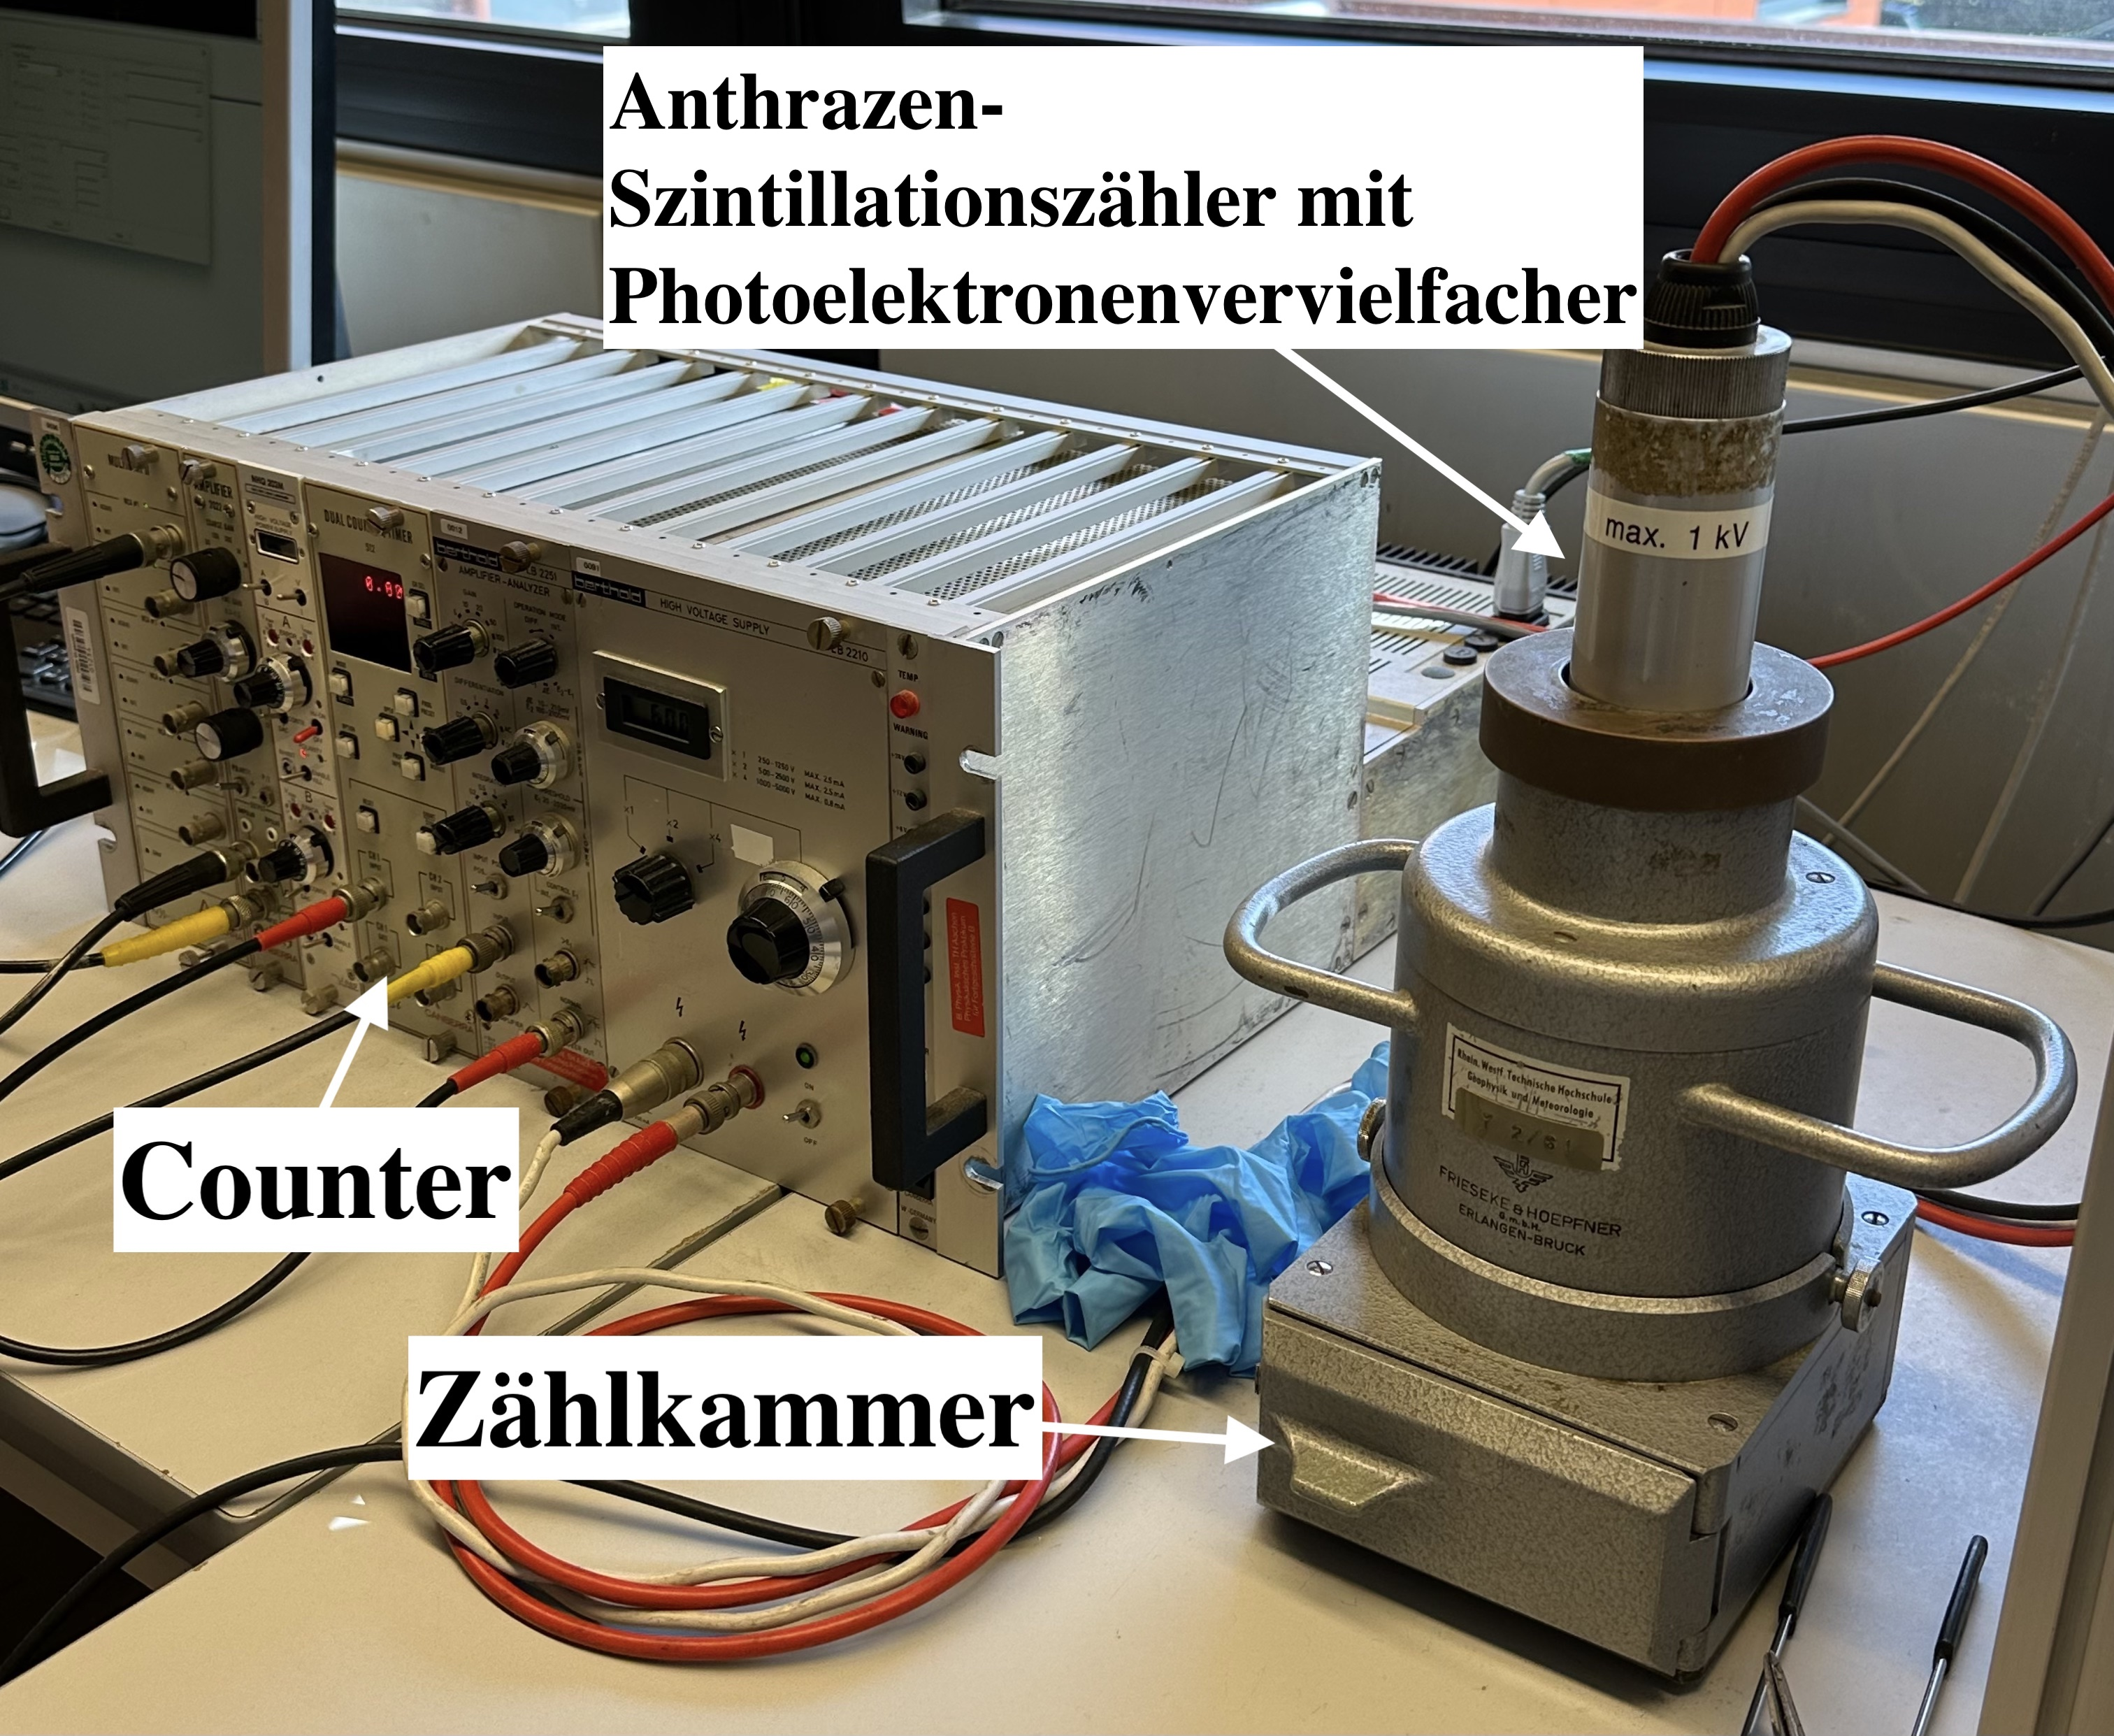
\includegraphics[width = 1\textwidth]{Bilder/Aufbau_Beta_Alu.jpeg}
\caption{\label{fig:Aubau_Beta_Alu} Aufbau}
    \end{figure}
\end{minipage} \hfill
\begin{minipage}{0.45\textwidth}

Der Aufbau besteht aus einem Anthrazen-Szintillationszähler unter dem sich eine Zählkammer befindet in der die $^{90}$Sr-Quelle eingeführt wird. Über der Quelle können Aluminiumplatten verschiedener Dicken eingesetzt werden. \\
Der Aufbau ist mit der Spannungsquelle und dem Zähler verbunden. 

\end{minipage}
\\
U = 650V, T = 60s

\begin{table}[h]
    \centering 
    \begin{tabular}{|l|c|c|c|c|c|}
        \hline 
        Alu. Absorber KennNr. & $5$ & $7$ & $9$ & $11$ & $13$  \\
        \hline
        \# Events & $87723$ & $83300$ & $75803$ & $61588$ & $40254$\\ 
        \hline \hline
        Alu. Absorber KennNr. & $15$ & $17$ & $19$ & $21$ & $23$ \\
        \hline
        \# Events & $20812$ & $7638$ & $3229$ & $673$ & $538$\\ 
        \hline \hline
        \multicolumn{6}{|l|}{Rauschmessung (ohne Bleibabsorber und Quelle):\quad $210$}\\
        \hline
    \end{tabular}
    \caption{Zählraten bei unterschiedlichen Bleidicken. Die Daten der Aluabsorber sind im Anhang C in \cite{Versuchsanleitung} zu finden.}
\end{table}


 


